\chapter{Hasil \textit{Usability Testing} Prototipe \textit{High-Fidelity} Iterasi Kedua}
\label{chpt:hasil_test_hifi2}

\section{Rangkuman Hasil SUS}

Jumlah partisipan adalah 5 orang.
Pertanyaan kuesioner SUS mengacu pada Lampiran \ref{subsec:sus}.

\begin{figure}[h]
  \centering
  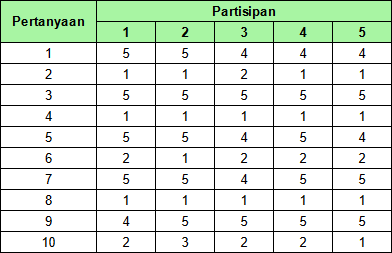
\includegraphics[width=0.7\textwidth]{hifi2/chart-sus.png}
\end{figure}


\section{Konversi Penghitungan Skor SUS dan SEQ}
Berikut adalah hasil konversi perhitungan skor SUS dan skor SEQ. Daftar \textit{task} mengacu pada Lampiran \ref{chpt:skenario_hifi1}.

\begin{figure}[h]
  \centering
  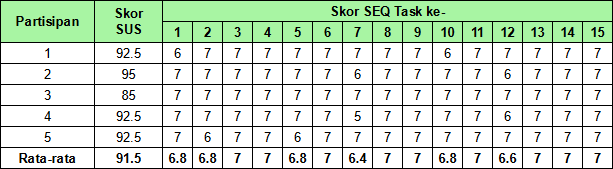
\includegraphics[width=\textwidth]{hifi2/chart-sus-seq.png}
\end{figure}

% \section{Waktu Penyelesaian Task}
% \normalsize

% Berikut adalah rangkuman waktu yang diperlukan setiap partisipan untuk menyelesaikan \textit{task} yang diberikan. Daftar \textit{task} mengacu pada Lampiran \ref{chpt:skenario_hifi1}.

% \begin{figure}[h]
%   \centering
%   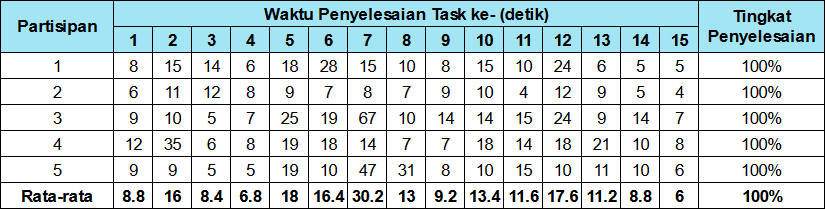
\includegraphics[width=\textwidth]{hifi2/chart-penyelesaian.png}
% \end{figure}

\newpage

\section{Konversi Perhitungan Skor IMI}

Berikut adalah rata-rata nilai 3 sub skala \textit{Intrinsic Motivation Inventory}. Daftar pertanyaan pada setiap sub skala IMI mengacu pada Lampiran \ref{subsec:imi}.

\begin{figure}[h]
  \centering
  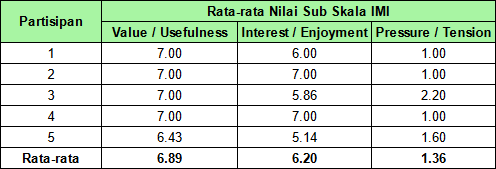
\includegraphics[width=0.95\textwidth]{hifi2/chart-imi.png}
\end{figure}